
\section{Реализация математической модели}\label{sec:ch2/sec5}

Сведем полученные выражения в единую систему:

\begin{equation}\label{eq:ch2/final_system}
    \begin{cases}
        \begin{alignedat}{2}
            \dot{x}               & = v                                                                                                                                                                                                   \\
            M\dot{v}              & = \mathbf{F}^T\mathbf{p} - p_\text{атм}(\mathbf{F}^T\mathbf{1}) - R_\text{тр}(v) - R_\text{оп}(x, v)                                                                                                  \\
            \dot{\mathbf{p}}      & = \frac{\gamma}{\mathbf{V}(\mathbf{x})} \odot (R\mathbf{T} \odot \mathbf{G} - \mathbf{p} \odot (\mathbf{F}v))                                                                                         \\
            \dot{\mathbf{T}}      & = \frac{\gamma-1}{\mathbf{m}C_v} \odot (R\mathbf{T} \odot \mathbf{G} \pm \mathbf{p} \odot (\mathbf{F}v))                                                                                              \\
            \mathbf{u}_\text{зад} & = \tau \dot{\mathbf{u}} + \mathbf{u}                                                                                                                                                                  \\
            \mathbf{G}            & = \psi(\mathbf{p}_\text{вх}, \mathbf{p}_\text{вых}) \odot \mathbf{C}_d \odot \mathbf{F}_\text{пр} \odot \mathbf{u} \odot \frac{\mathbf{p}_\text{вх}}{\sqrt{R\mathbf{T}_\text{вх}}}                    \\
            R_\text{тр} &= \sigma_0 z + \sigma_1 \dot{z} + \sigma_2 v                                                                                                                              \\
            \dot{z} &= v - \frac{\sigma_0 |v|}{g(v)}z \\
            R_\text{оп}           & = k_\text{оп}(x - x_\text{мин})\cdot \frac{1}{1 + e^{-\alpha(x - x_\text{мин})}} + k_\text{оп}(x - x_\text{макс})\cdot \frac{1}{1 + e^{-\alpha(x - x_\text{макс})}}                                   \\
        \end{alignedat}
    \end{cases}
\end{equation}

Представим данную систему в виде функциональной блок-схемы, представленной на рисунке \ref{fig:ch2/block_diagram}.

\begin{figure}[ht]
    \centerfloat{
        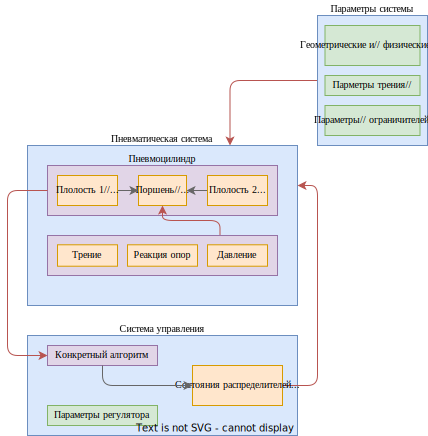
\includegraphics[]{part2/diagrams/pneumatic_actuator_functional_block_diagram.pdf}
    }
    \caption{Функциональная блок-схема математической модели электропневматического привода}
    \label{fig:ch2/block_diagram}
\end{figure}

В процессе исследования осуществлена программная реализация математической модели пневматического привода с применением объектно-ориентированного подхода.
При разработке программного комплекса использован язык программирования Python, обеспечивающий необходимую функциональность для численного моделирования и
обработки результатов. Архитектура программного комплекса базируется на принципах модульности и инкапсуляции, что обеспечивает высокую степень гибкости при
модификации отдельных компонентов системы.

Центральным элементом реализации является класс \texttt{PneumaticCylinder}, инкапсулирующий математическую модель пневматического привода.
В данном классе реализована система дифференциальных уравнений, описывающих динамику привода, включая уравнения движения поршня,
термодинамические процессы в рабочих полостях и динамику переключения распределителей. Математическая модель дополнена отдельными
классами для описания нелинейных эффектов: \texttt{FrictionModel} -- для моделирования сил трения и \texttt{StopForce} -- для учета ограничений хода поршня.

Численное интегрирование системы дифференциальных уравнений осуществляется с использованием метода BDF (Backward Differentiation Formula),
реализованного в библиотеке \texttt{scipy.integrate}. Выбор данного метода обусловлен жёсткостью исследуемой системы дифференциальных
уравнений. Для повышения эффективности численного интегрирования реализовано аналитическое вычисление матрицы Якоби, что позволяет существенно
сократить вычислительные затраты и повысить численную стабильность решения.

Визуализация результатов моделирования реализована с применением библиотеки Matplotlib, обеспечивающей
построение графиков временных зависимостей основных параметров системы: перемещения и скорости поршня, давлений и температур
в полостях цилиндра, состояний распределителей. При этом программный комплекс предусматривает возможность экспорта результатов
в различные форматы для последующей обработки и анализа.

Разработанная программная реализация обеспечивает возможность эффективного проведения вычислительных экспериментов,
параметрической оптимизации и анализа динамических характеристик пневматического привода. Модульная структура программного
комплекса позволяет легко модифицировать отдельные компоненты системы и интегрировать новые алгоритмы управления.